%\documentclass[xcolor=dvipsnames,compress,handout]{beamer}
\documentclass[xcolor=dvipsnames,compress]{beamer}
\usepackage[utf8]{inputenc}
\usepackage[ngerman,english]{babel}
\usepackage{pgf}
\usepackage{graphicx}
\graphicspath{ {images/} }
\usepackage[absolute,overlay]{textpos}
\usepackage{xcolor}
\usepackage{comment}
%\usepackage{algorithm2e}
%\usepackage{algorithmic}
\usepackage{xpatch}
\usepackage{tabularx}
\usepackage[export]{adjustbox}
\usepackage{tikz}
\usepackage{pgffor}
\usepackage{blindtext}

% DESIGN
\definecolor{RUBblue}{rgb}{0,0.21,0.38}
\definecolor{AIblue}{rgb}{0,0.57,0.87}

% DO NOT ASK WHAT HAPPENS HERE
% Okay...
\useoutertheme[subsection=false]{miniframes}
\usecolortheme{beaver}
\beamertemplatenavigationsymbolsempty
\setbeamertemplate{footline}{%
    \begin{beamercolorbox}[wd=\paperwidth,ht=0ex,left]{default}
        %\insertauthor\hfill\insertframenumber%
        \colorbox{AIblue}{\vphantom{2cm}\hspace{14cm}}
    \end{beamercolorbox}
}
\setbeamercolor{item}{fg=RUBblue}
\setbeamercolor{title}{fg=Black}
\setbeamercolor{frametitle}{fg=Black}
\setbeamerfont{title}{size=\large}
\setbeamertemplate{itemize items}[square]
\setbeamercolor{section in head/foot}{bg=AIblue}
\setbeamerfont{footline}{size=\fontsize{15}{12}\selectfont}


\xpatchcmd{\itemize}
  {\def\makelabel}
  {\setlength{\itemsep}{0.2cm}\def\makelabel}{}{}

 
\addtobeamertemplate{frametitle}{}{%
\begin{textblock*}{100mm}(1.05\textwidth,0.535cm)

\includegraphics[height=0.975cm,width=0.98cm]{logo-rub.png}
\end{textblock*}}

% COMMANDS
\newcommand\NEWLINECOMMENT[1]{\STATE\STATE/* #1 */}
\newcommand\Only[2]{\only<#1|handout:#1>{#2}}
\newcommand\overlayImage[6]{
	\only<#1|handout:#2>{
		\begin{textblock*}{\textwidth}(#3cm,#4cm)
			\frame{
				\includegraphics[width=#5\textwidth]{#6}
			}
		\end{textblock*}
	}
}


% TITLEPAGE
\title{\textbf{Deep Convolutional Networks}}
\author{Christian Andreas Mielers\\Phil Yannick Schrör}
\institute{Ruhr-University Bochum\\Institute for Neural Computation\\Study Project}
\date{24th of February 2016}
 
\begin{document}
\section{Welcome}
\subsection{Welcome}
\maketitle

\section{Convolutional Neural Networks}
\subsection{Convolutional Neural Networks}

\frame{
	\frametitle{Convolutional Neural Networks}
	\begin{columns}
		\column{0.5\textwidth}
			\begin{itemize}
				\item Learns the weights of convolutional filters
				\item Exploits spatial structure in the input
				\item Convolving entire input with filter implies shared weights
				\item Reduced amount of weights allows lots of filters
				\item Filters specific to color channels
			\end{itemize}
		\column{0.5\textwidth}
			\includegraphics<1>[width=\textwidth]{dense_layer}
			\includegraphics<2>[width=\textwidth]{convolutional_layer}
			\includegraphics<3>[width=\textwidth]{color_mapping}
	\end{columns}
}
%TODO pooling layers

\frame{
	\frametitle{Network Structure}
	\begin{textblock*}{1.1\textwidth}(0.5cm,2.9cm)
		\footnotesize{
			\begin{tabularx}{\textwidth}{cp{0.16\linewidth}p{0.4\linewidth}X}
			\textbf{Layer} & \textbf{Type} & \textbf{Configuration} & \textbf{Activation function} \\
			& & & \\
			\hline
			& & & \\
			0 & Convolutional & 100 filters of size $7\times7$ per channel & $\tanh$ \\
			1 & Max Pooling & Pool size $2\times2$ & - \\
			2 & Convolutional & 150 filters of size $4\times4$ per channel & $\tanh$ \\
			3 & Max Pooling & Pool size $2\times2$ & - \\
			4 & Convolutional & 250 filters of size $4\times4$ per channel & $\tanh$ \\
			5 & Max Pooling & Pool size $2\times2$ & - \\
			6 & Dense & 300 neurons & $\tanh$ \\
			7 & Dense & \#classes neurons & softmax
			\end{tabularx}
		}
		%TODO Add image of tanh function somewhere
	\end{textblock*}
}

\section{GTSRB}
\subsection{GTSRB}

\frame{
	\frametitle{German Traffic Sign Recognition Benchmark}
	\begin{columns}
		\column{0.54\textwidth}
			\begin{itemize}
				\item Dataset of traffic signs taken while on the road
				\item 39209 training and 12630 test images in 43 classes
				\item Multiple images per sign
				\item Images contain a 10\% border around the sign
				\item Annotations provide precise sign locations
					\begin{itemize}
						\item We cropped out just the sign
					\end{itemize}
			\end{itemize}
		\column{0.5\textwidth}
			\centering
			\includegraphics<1>[width=0.4\textwidth]{gtsrb_00002_00029}
			\includegraphics<2>[width=0.4\textwidth]{gtsrb_00002_00029_border}
			
			\includegraphics<1>[width=0.4\textwidth]{gtsrb_00013_00029}
			\includegraphics<2>[width=0.4\textwidth]{gtsrb_00013_00029_border}
			
			\includegraphics<1>[width=0.4\textwidth]{gtsrb_00029_00029}
			\includegraphics<2>[width=0.4\textwidth]{gtsrb_00029_00029_border}
	\end{columns}
}

\frame{
	\frametitle{Simple Setup}
	\begin{columns}
		\column{0.5\textwidth}
			\begin{itemize}
				\item Input size $48 \times 48$
				\item Contrast normalization
				\item Gradient descent on batches of 16 images
				\item Training time $\approx 10h$
			\end{itemize}
		\column{0.5\textwidth}
			\centering
			
\includegraphics[width=0.4\textwidth]{gtsrb_00019_00004_00029}
			
			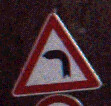
\includegraphics[width=0.4\textwidth]{gtsrb_00019_00004_00029_contr}
	\end{columns}
}

\begin{frame}
	\frametitle{Results on GTSRB}
	\begin{columns}
		\column{0.35\textwidth}
			\begin{itemize}
				\item Levels off after 6 epochs
				\item Peaks at $\approx 0.9660$ accuracy after 14 epochs
			\end{itemize}
		\column{0.65\textwidth}
			\centering
			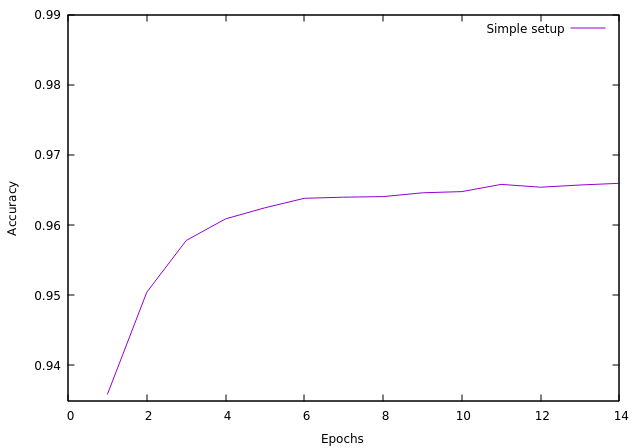
\includegraphics[width=\textwidth]{gtsrb_results_1}
	\end{columns}
\end{frame}

\begin{frame}
	\frametitle{Filter Visualization}
	
	\only<1>{
		\begin{figure}
			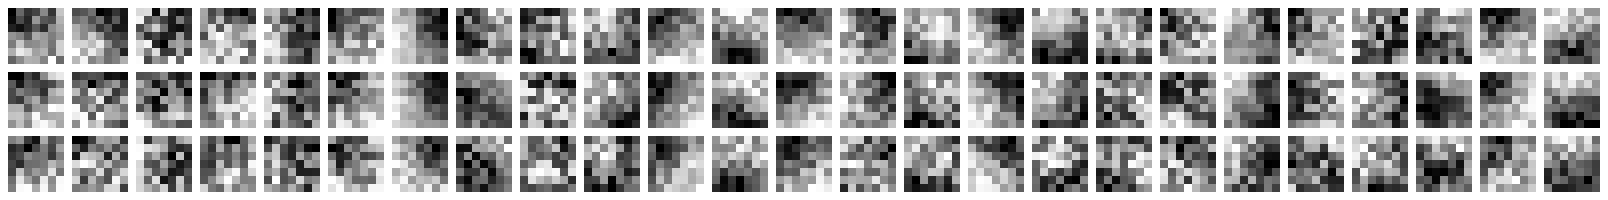
\includegraphics[width=\textwidth]{filter_visualizations/gtsrb_nomorph_filters_0}
			\caption{Filters on the first convolutional layer}
		\end{figure}
		
		\begin{itemize}
			\item Visible structure
			\item Mostly edge and corner detectors
			\item Similarity across color channels
				\begin{itemize}
					\item Indicates color independence
				\end{itemize}
		\end{itemize}
	}
	
	\only<2>{
		\begin{figure}
			\includegraphics<2>[width=\textwidth]{filter_visualizations/gtsrb_nomorph_filters_2}
			\caption{Filters on the second convolutional layer}
		\end{figure}
		
		\begin{itemize}
			\item Notably less structure
			\item Might indicate higher specialization due to more filters
		\end{itemize}
	}
	
	\only<3>{
		\begin{figure}
			\includegraphics<3>[width=\textwidth]{filter_visualizations/gtsrb_nomorph_filters_4}
			\caption{Filters on the third convolutional layer}
		\end{figure}
		
		\begin{itemize}
			\item No qualitative difference from second convolutional layer
		\end{itemize}
	}
\end{frame}

\frame{
	\frametitle{Input Distortions}
	\begin{textblock*}{1.1\textwidth}(-0.2cm,1.8cm)
		\begin{itemize}
			\item Random distortions  before each epoch
			\item Should improve generalization
			\item They consist of affine transformations
		\end{itemize}
	\end{textblock*}
	\begin{textblock*}{1.1\textwidth}(6.7cm,1.8cm)
		\begin{itemize}
			\item Translation (10\% of image size)
			\item Rotation (5 degrees)
			\item Scaling (10\% of image size)
		\end{itemize}
	\end{textblock*}
	\begin{textblock*}{1.1\textwidth}(0.3cm,4.0cm)
		\begin{figure}
			\centering
			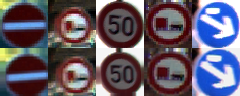
\includegraphics[width=0.8\textwidth]{distortions.png}
		\end{figure}
	\end{textblock*}
}

\frame{
	\frametitle{Results with Distortions}
	\begin{columns}
		\column{0.35\textwidth}
			\begin{itemize}
				\item Peaks at $\approx 0.9774$ accuracy after 14 epochs
				\item Notable improvement
				\item More volatility
			\end{itemize}
		\column{0.65\textwidth}
			\centering
			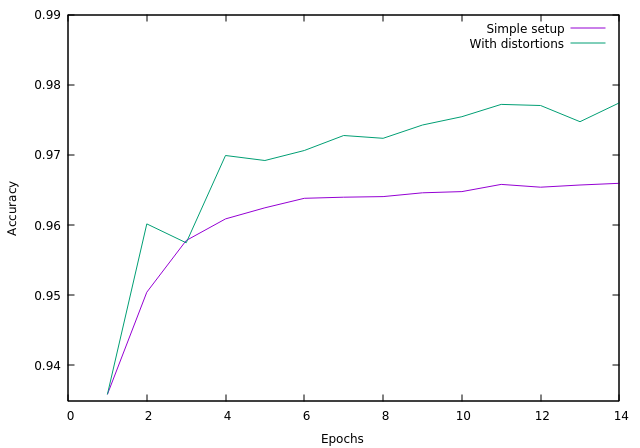
\includegraphics[width=\textwidth]{gtsrb_results_2}
	\end{columns}
}

\frame{
	\frametitle{RELU Activation Function}
	\begin{columns}
		\column{0.5\textwidth}
			\begin{itemize}
				\item Alternative activation function
				\item Efficient computation
				\item Forward pass about $2\times$ faster
			\end{itemize}
		\column{0.5\textwidth}
			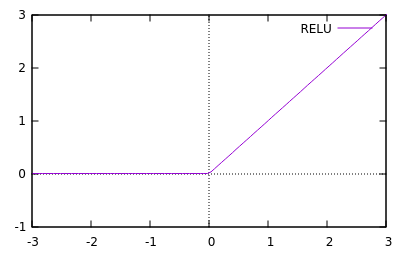
\includegraphics[width=\textwidth]{relu}
	\end{columns}
}

\frame{
	\frametitle{Results with RELU}
	\begin{columns}
		\column{0.35\textwidth}
			\begin{itemize}
				\item Peaks at $\approx 0.9803$ accuracy after 10 epochs
				\item Slightly better sometimes
				\item Very erratic development
				\item Use of tanh activation function in further considerations
			\end{itemize}
		\column{0.65\textwidth}
			\centering
			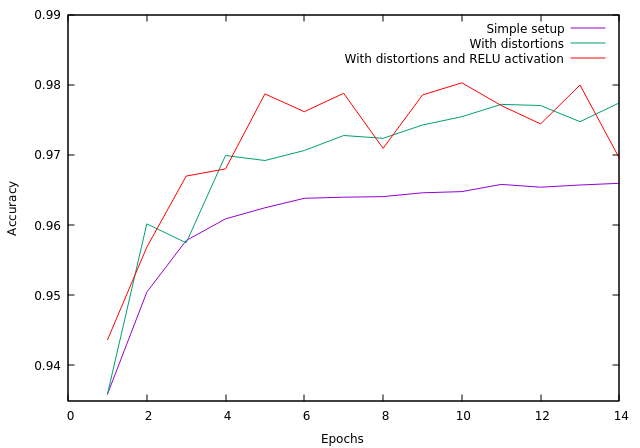
\includegraphics[width=\textwidth]{gtsrb_results_3}
	\end{columns}
}

\frame{
	\frametitle{Missclassified images}
	\begin{figure}
		\centering
		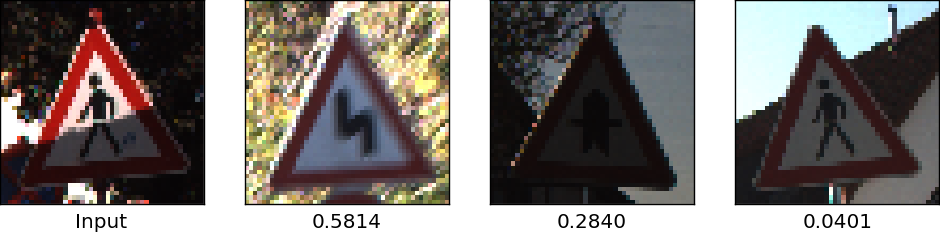
\includegraphics[width=0.85\textwidth]{gtsrb_mistakes/mistake_fussgaenger.png}
		
		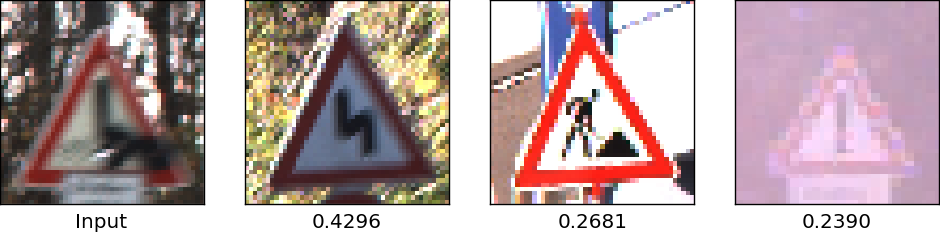
\includegraphics[width=0.85\textwidth]{gtsrb_mistakes/mistake_gefahrenstelle.png}
		
		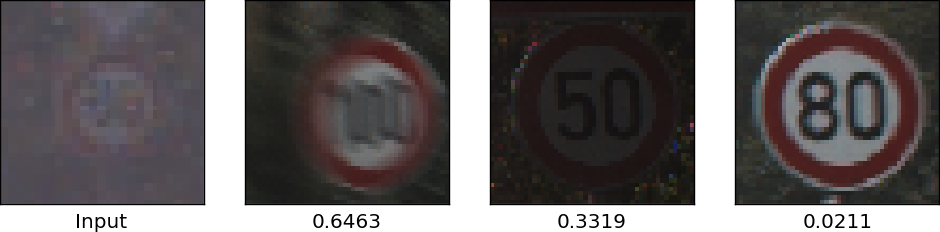
\includegraphics[width=0.85\textwidth]{gtsrb_mistakes/mistake_limit_unknown.png}
	\end{figure}
}

\section{Filter Reuse}
\subsection{Filter Reuse}

\frame{
	\frametitle{Filter Reuse}
	\begin{itemize}
		\item How well do the GTSRB filters generalize?
		\item Randomly initialize new network with same structure
		\item Copy GTSRB filters to the new network
		\item Train only the fully connected layers!
	\end{itemize}
}

\frame{
	\frametitle{COIL100}
	\begin{textblock*}{1.09\textwidth}(0.5cm,1.6cm)
		\begin{figure}
			\centering
			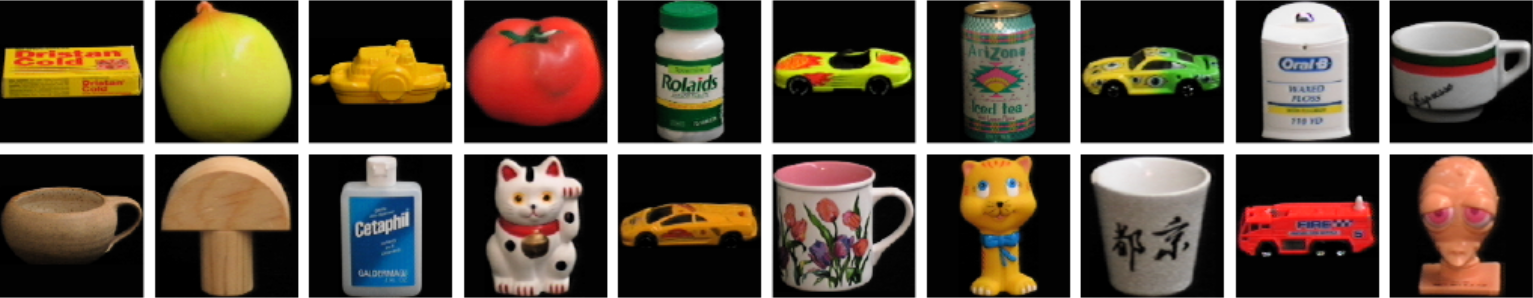
\includegraphics[width=\textwidth]{coil100.png}
		\end{figure}
	\end{textblock*}
	\begin{textblock*}{1.1\textwidth}(0.5cm,4.55cm)
		\begin{itemize}
			\item Columbia Object Image Library 100 $\Rightarrow$ COIL100
			\item 100 different objects
			\item Objects placed on a black turntable
			\item One photo each time the object has turned by $5^\circ$
			\item 72 images per object, 7200 images in total
			\item Random separation into 58 training and 14 test images per object
		\end{itemize}
	\end{textblock*}
}

\frame{
	\frametitle{COIL100 --- GTSRB Filters Results}
	\begin{textblock*}{1.1\textwidth}(0.3cm,1.1cm)
		\begin{figure}
			\centering
			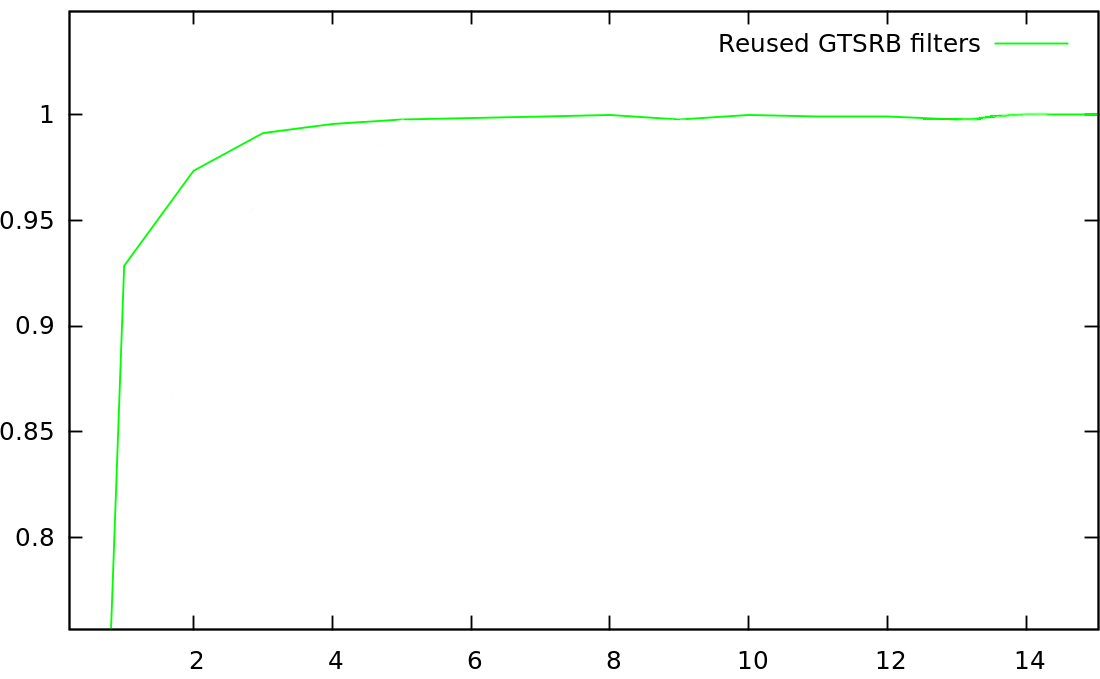
\includegraphics[width=1.02\textwidth]{coil100_results_gtsrb_only.png}
		\end{figure}
	\end{textblock*}
	\Only{2}{
		\begin{textblock*}{1.1\textwidth}(1.8cm,4.5cm)
			\begin{itemize}
				\item Monotonic increase until the 8th epoch
				\item Random distortions $\Rightarrow$ Slight decreases
				\item One epoch takes around 5 minutes
				\item Very good results in a short time
			\end{itemize}
		\end{textblock*}
	}
	\begin{textblock*}{1.1\textwidth}(9.8cm,4.2cm)
		\tiny
		\begin{tabular}{|r|r|}
			\hline
			Epoch & Accuracy\\ \hline
			1 & 0.9286\\
			2 & 0.9736\\
			3 & 0.9914\\
			4 & 0.9957\\
			5 & 0.9979\\
			6 & 0.9986\\
			7 & 0.9993\\
			8 & 1.0000\\
			9 & 0.9979\\
			10 & 1.0000\\
			11 & 0.9993\\
			12 & 0.9993\\
			13 & 0.9979\\
			14 & 1.0000\\
			15 & 1.0000\\ \hline
		\end{tabular}
	\end{textblock*}
}

\frame{
	\frametitle{COIL100 --- Original filters}
	\begin{itemize}
		\item What are the advantages of this approach?
		\item We need data for a comparison
		\item Train a new network conventionally on COIL100
		\item Call the filters which are created this way \emph{original}
		\item Compare training time and results!
	\end{itemize}
}


\frame{
	\frametitle{COIL100 --- Original Filters Results}
	\begin{textblock*}{1.1\textwidth}(0.3cm,1.1cm)
		\begin{figure}
			\centering
			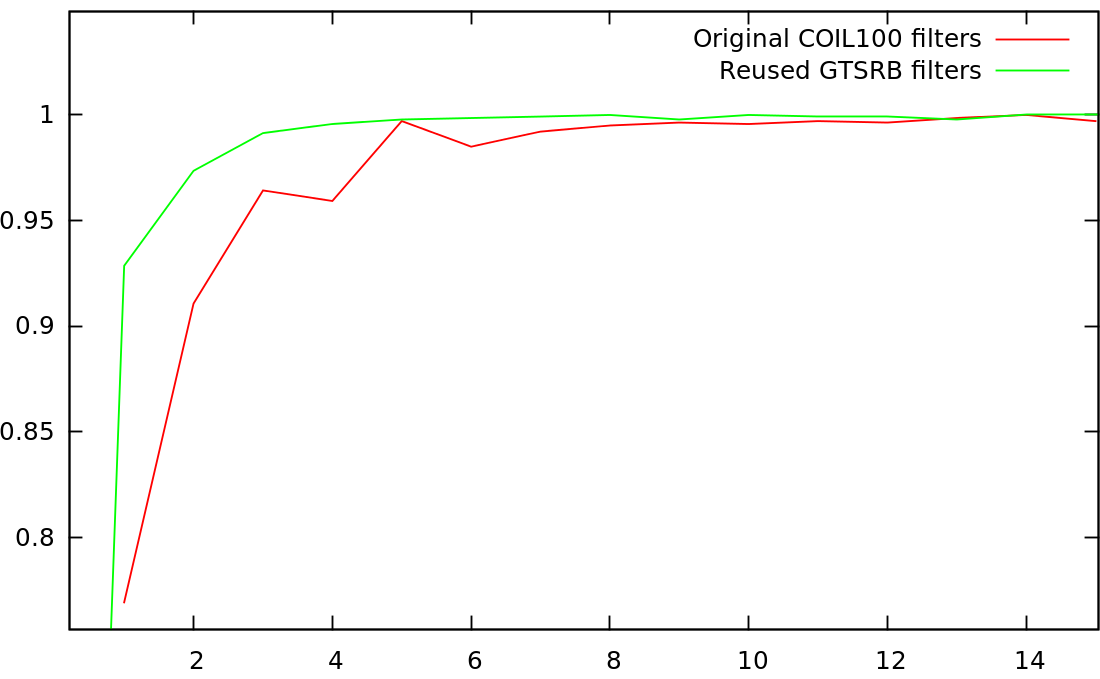
\includegraphics[width=1.02\textwidth]{coil100_results.png}
		\end{figure}
	\end{textblock*}
	\Only{2}{
		\begin{textblock*}{0.5\textwidth}(3.1cm,4.5cm)
			\begin{itemize}
				\item GTSRB filters dominate
				\item Similar results in the end
				\item Training time: $\sim$90min
				\item What do the original filters look like?
			\end{itemize}
		\end{textblock*}
	}
	\begin{textblock*}{1.1\textwidth}(8.8cm,4.25cm)
		\tiny
		\begin{tabular}{|r|rr|}
			\hline
			Epoch & GTSRB & Original\\ \hline
			1 & 0.9286 & 0.7693\\
			2 & 0.9736 & 0.9107\\
			3 & 0.9914 & 0.9643\\
			4 & 0.9957 & 0.9593\\
			5 & 0.9979 & 0.9971\\
			6 & 0.9986 & 0.9850\\
			7 & 0.9993 & 0.9921\\
			8 & 1.0000 & 0.9950\\
			9 & 0.9979 & 0.9964\\
			10 & 1.0000 & 0.9957\\
			11 & 0.9993 & 0.9971\\
			12 & 0.9993 & 0.9964\\
			13 & 0.9979 & 0.9986\\
			14 & 1.0000 & 1.0000\\
			15 & 1.0000 & 0.9971\\ \hline
		\end{tabular}
	\end{textblock*}
}

\frame{
	\frametitle{COIL100 --- What do the original filters look like?}
	\begin{textblock*}{1.1\textwidth}(0.3cm,1.3cm)
		\begin{figure}
			\centering
			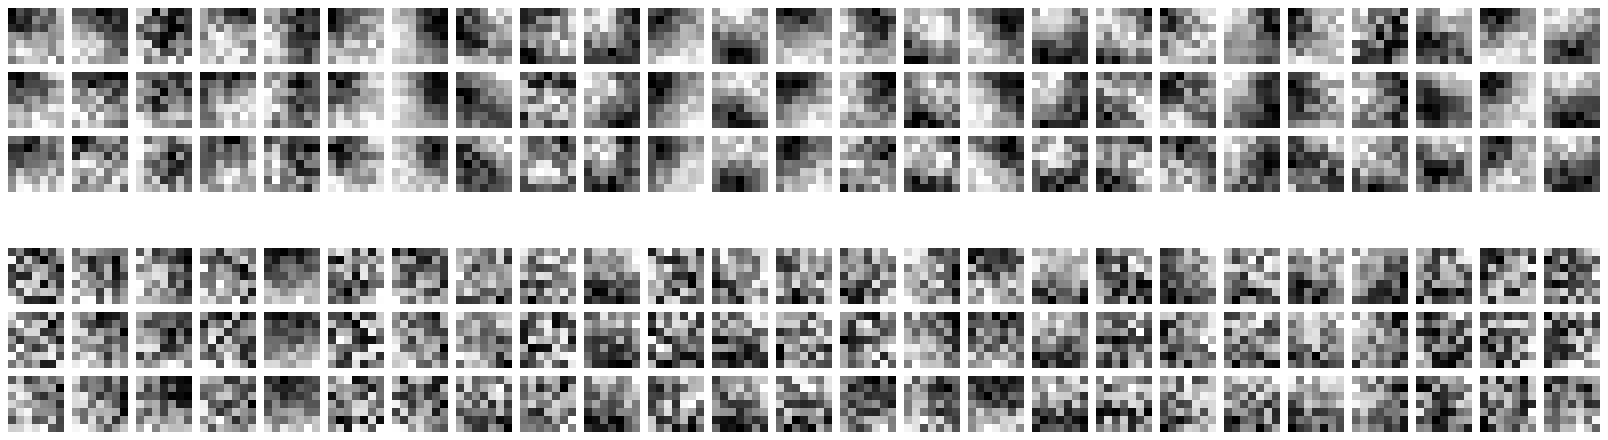
\includegraphics[width=1.03\textwidth]{gtsrb_vs_coil_filters.png}
		\end{figure}
	\end{textblock*}
	\begin{textblock*}{1.2\textwidth}(-0.1cm,5.3cm)
		\begin{itemize}
			\item The spatial structure is not as distinctive as the one of the GTSRB filters
			\item One cannot expect a good generalization behavior of the COIL100 filters
			\item Maybe the CNN is oversized for the task
			\item The original filters exhibit more differences between the color channels
			\item Long training time, but probably overfitted filters
		\end{itemize}
	\end{textblock*}
}

\frame{
	\frametitle{INRIA}
	\begin{textblock*}{1.09\textwidth}(2.8cm,1.35cm)
		\begin{figure}
			\centering
			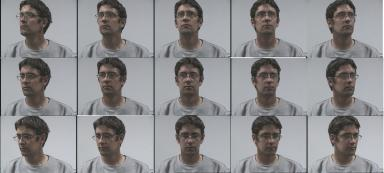
\includegraphics[width=0.65\textwidth]{inria_different_angles.jpg}
		\end{figure}
	\end{textblock*}
	\begin{textblock*}{0.44\textwidth}(0.0cm,1.6cm)
		\begin{itemize}
			\item Just luck?
			\item French Institute for Reseach in Computer Science and Automation (INRIA): Head Pose Image Database
			\item Details matter
		\end{itemize}
	\end{textblock*}
	\begin{textblock*}{1.2\textwidth}(0.0cm,5.6cm)
		\begin{itemize}
			\item 15 persons, 2 series per person, 93 images per series
			\item Gradual change of head position (with or without features like glasses)
			\item 186 images $\Rightarrow$ 149 training and 37 test images
			\item Images were not cropped
			\item Color is not a discriminative feature
		\end{itemize}
	\end{textblock*}
}

\frame{
	\frametitle{INRIA --- GTSRB Filters Results}
	\begin{textblock*}{1.06\textwidth}(0.37cm,1.1cm)
		\begin{figure}
			\centering
			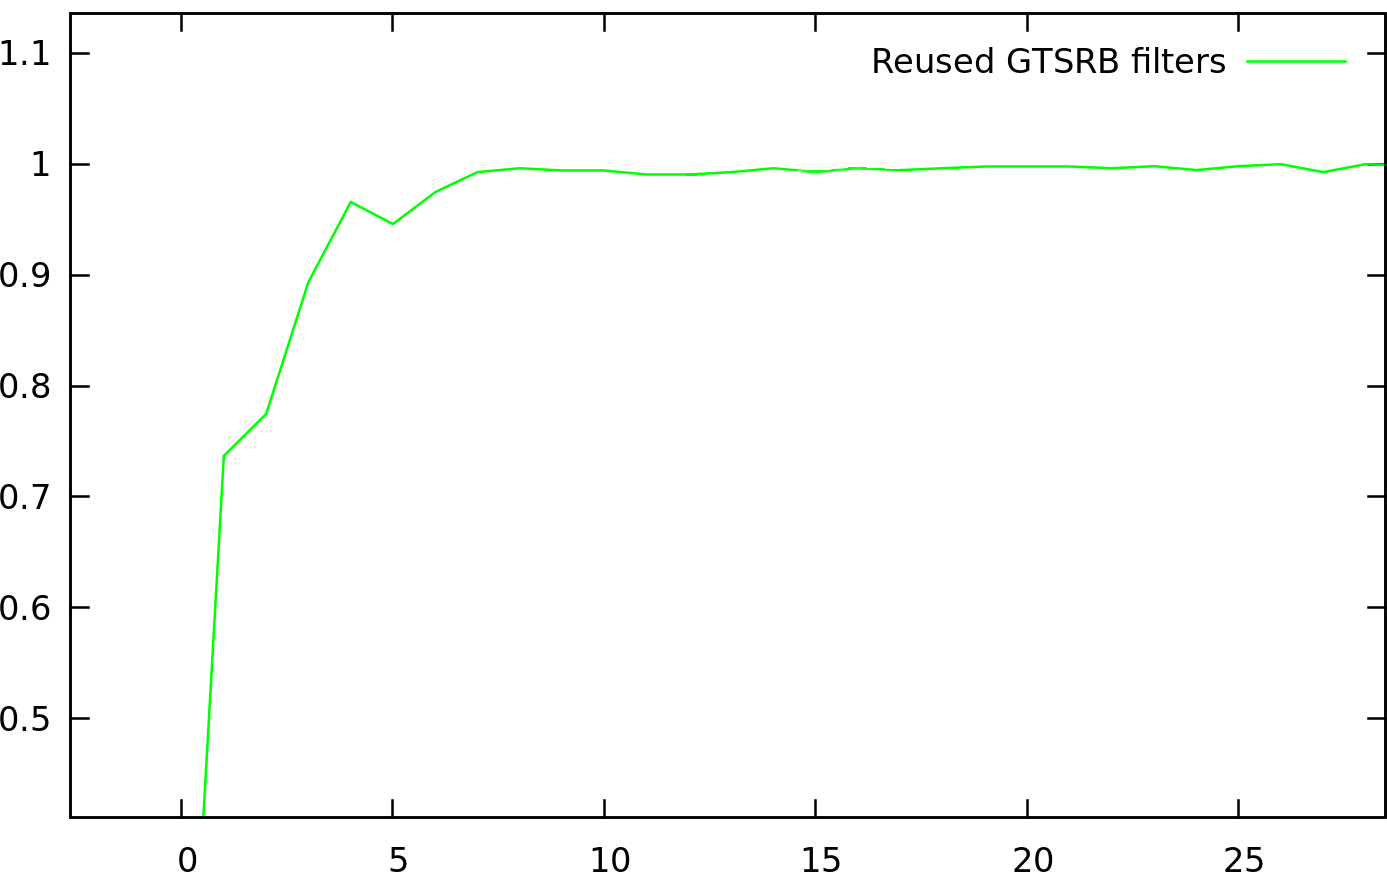
\includegraphics[width=1.02\textwidth]{inria_results_only_gtsrb.png}
		\end{figure}
	\end{textblock*}
	\Only{2}{
		\begin{textblock*}{1.1\textwidth}(3.2cm,4.6cm)
			\begin{itemize}
				\item Over 99\% after 7 epochs
				\item Training time $<$ 2 minutes
				\item Good results in little time
			\end{itemize}
		\end{textblock*}
	}
	\begin{textblock*}{1.1\textwidth}(9.5cm,3.75cm)
		\tiny
		\begin{tabular}{|r|r|}
			\hline
			Epoch & Accuracy\\ \hline
			01 & 0.7369\\
			02 & 0.7748\\
			03 & 0.8937\\
			04 & 0.9658\\
			05 & 0.9459\\
			06 & 0.9748\\
			07 & 0.9928\\
			08 & 0.9964\\
			09 & 0.9946\\
			10 & 0.9946\\
			11 & 0.9910\\
			12 & 0.9910\\
			13 & 0.9928\\
			14 & 0.9964\\
			15 & 0.9928\\
			16 & 0.9964\\
			17 & 0.9946\\ \hline
		\end{tabular}
	\end{textblock*}
}

\frame{
	\frametitle{INRIA --- GTSRB Filters Results}
	\begin{textblock*}{1.0\textwidth}(0.8cm,1.5cm)
		\begin{figure}
			\centering
			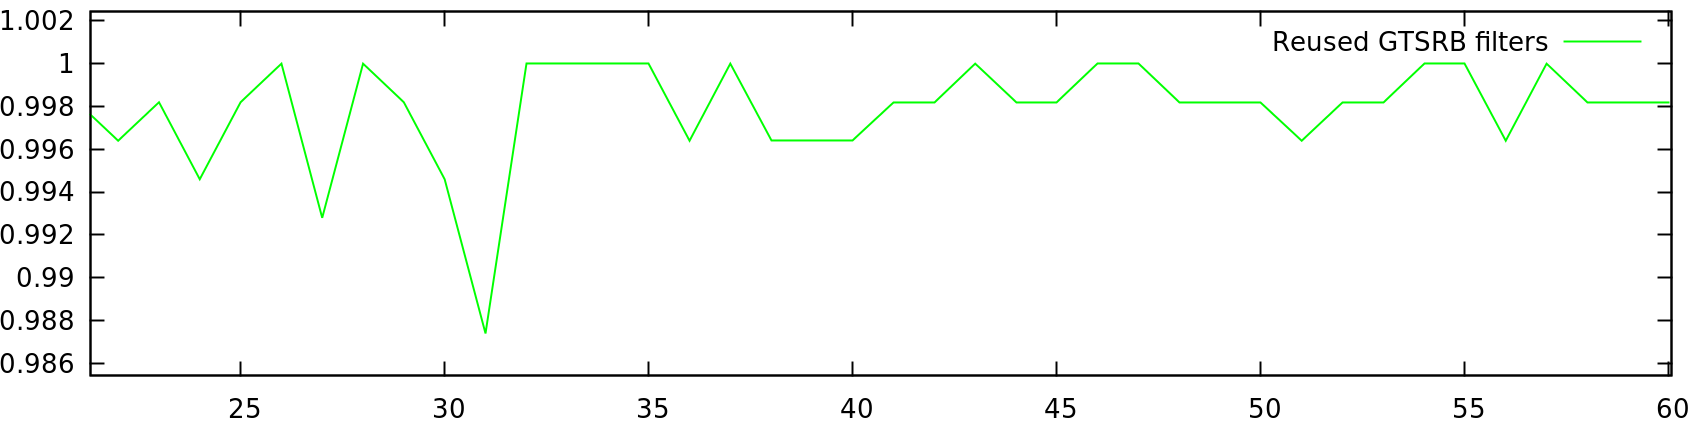
\includegraphics[width=1.02\textwidth]{inria_results_late_gtsrb.png}
		\end{figure}
	\end{textblock*}
	\begin{textblock*}{1.1\textwidth}(0.2cm,4.75cm)
		\begin{itemize}
			\item Low training cost $\Rightarrow$ Many epochs
			\item Accuracy under 99.5\% only 3 times after first 20 epochs
		\end{itemize}
	\end{textblock*}
	\begin{textblock*}{1.06\textwidth}(0.7cm,6.0cm)
		\begin{figure}
			\centering
			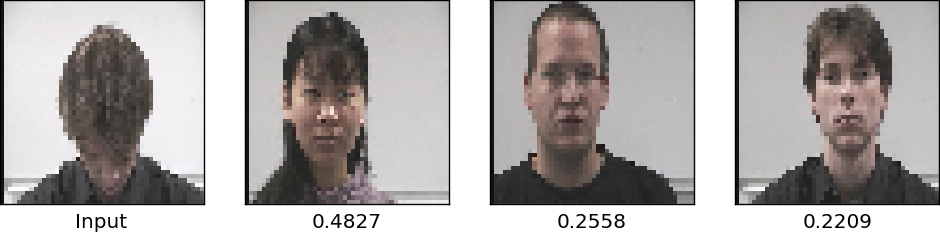
\includegraphics[width=0.9\textwidth]{mistake_looking_down.png}
		\end{figure}
	\end{textblock*}
}

\frame{
	\frametitle{INRIA --- Original Filters Results}
	\begin{textblock*}{1.06\textwidth}(0.3cm,1.1cm)
		\begin{figure}
			\centering
			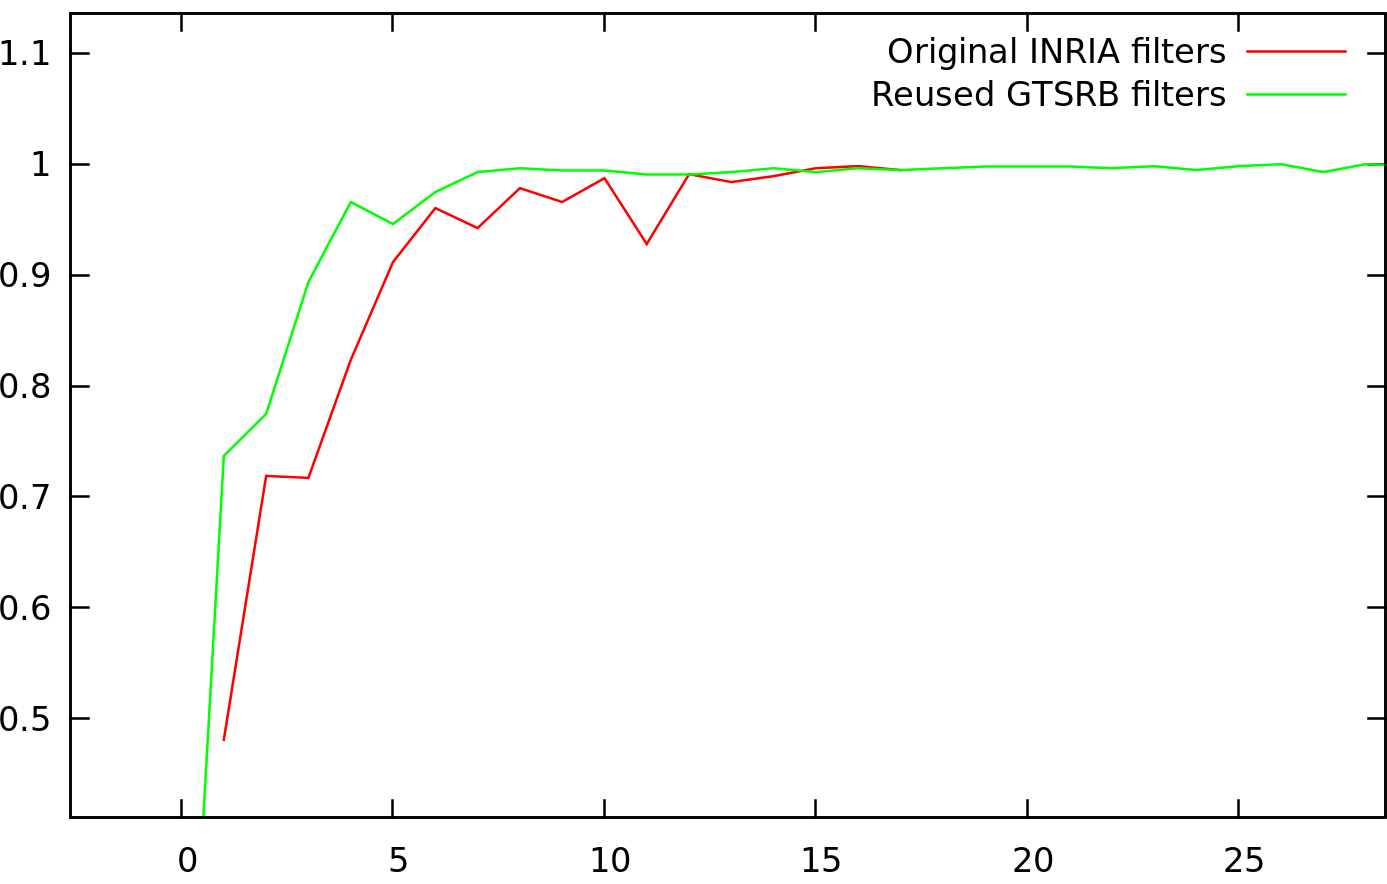
\includegraphics[width=1.\textwidth]{inria_results.png}
		\end{figure}
	\end{textblock*}
	\Only{2}{
		\begin{textblock*}{0.5\textwidth}(3.1cm,4.5cm)
			\begin{itemize}
				\item GTSRB filters dominate
				\item Similar results in the end
				\item Training time: $\sim$30m
				\item What do the original filters look like?
			\end{itemize}
		\end{textblock*}
	}
	\begin{textblock*}{1.1\textwidth}(8.2cm,3.6cm)
		\tiny
		\begin{tabular}{|r|rr|}
			\hline
			Epoch & GTSRB & Original\\ \hline
			01 & 0.7369 & 0.4811\\
			02 & 0.7748 & 0.7189\\
			03 & 0.8937 & 0.7171\\
			04 & 0.9658 & 0.8234\\
			05 & 0.9459 & 0.9117\\
			06 & 0.9748 & 0.9604\\
			07 & 0.9928 & 0.9423\\
			08 & 0.9964 & 0.9784\\
			09 & 0.9946 & 0.9658\\
			10 & 0.9946 & 0.9874\\
			11 & 0.9910 & 0.9279\\
			12 & 0.9910 & 0.9910\\
			13 & 0.9928 & 0.9838\\
			14 & 0.9964 & 0.9892\\
			15 & 0.9928 & 0.9964\\
			16 & 0.9964 & 0.9982\\
			17 & 0.9946 & 0.9946\\ \hline
		\end{tabular}
	\end{textblock*}
}

\frame{
	\frametitle{INRIA --- What do the original filters look like?}
	\begin{textblock*}{1.1\textwidth}(0.3cm,1.3cm)
		\begin{figure}
			\centering
			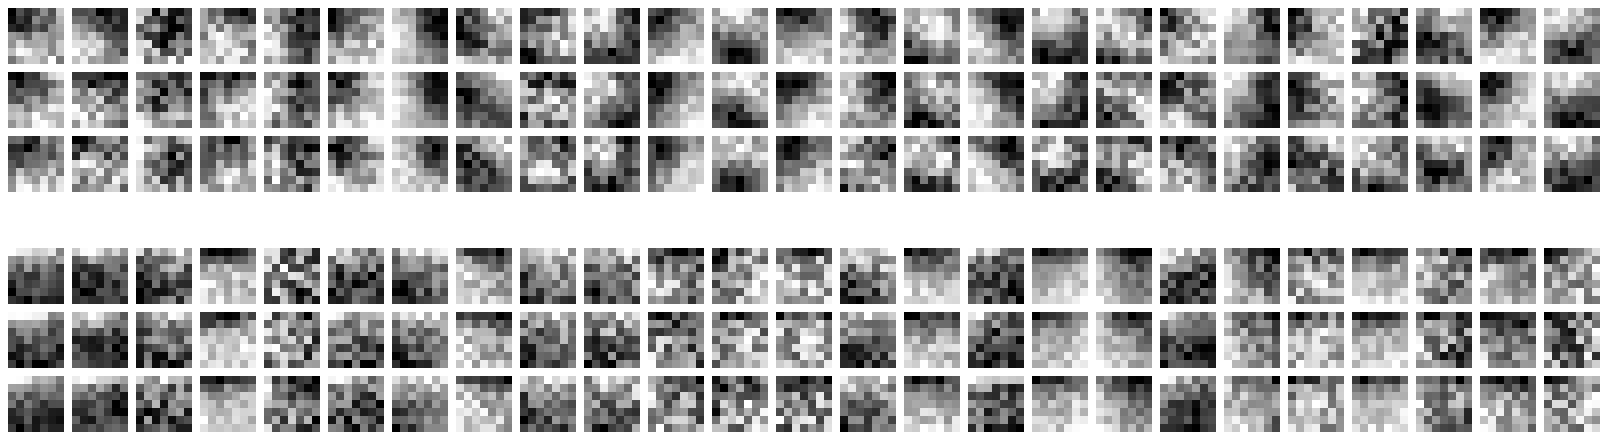
\includegraphics[width=1.03\textwidth]{gtsrb_vs_inria_filters.png}
		\end{figure}
	\end{textblock*}
	\begin{textblock*}{1.2\textwidth}(-0.1cm,5.1cm)
		\begin{itemize}
			\item No significant qualitative difference between GTSRB and INRIA filters. Mabye, the INRIA filters are slightly more noisy
			\item Almost no color dependence!
			\item Both filters sets will probabily generalize well
			\item INRIA filters yield 99.79\% after 10 epochs on COIL100
			\item GTSRB 10h vs. INRIA 0.5h per epoch
		\end{itemize}
	\end{textblock*}
}


\section{Conclusion}
\subsection{Conclusion}

\frame{
	\frametitle{Conclusion}
	\begin{itemize}
		\item Convolutional Networks use parameters efficiently
		\item Filters on first layer are well structured
			\begin{itemize}
				\item Filters on deeper layers look more noisy
			\end{itemize}
		\item Random distortions of input greatly improve generalization
		\item RELU activation is fast and sometimes better
			\begin{itemize}
				\item At the cost of reliability
			\end{itemize}
		\item Occlusion and low image quality impede classification
		\item Very good results with GTSRB filters on COIL100 and INRIA
		\item COIL100 filters: noisy, INRIA filters: like GTSRB filters
		\item Reliable classifiers can be constructed in little time
	\end{itemize}
}

\section{Questions?}
\subsection{Questions?}

\frame{
	\frametitle{Questions?}
	\begin{figure}[h!]
		\begin{textblock*}{\textwidth}(1.0cm,2.3cm)
			%Questions? \\
			\vspace{0.3cm}
			\frame{
				
\includegraphics[width=7cm]{fragen.png}
			}
		\end{textblock*}
	\end{figure}
}

\end{document}

